\documentclass{standalone}
% includes
\usepackage{pgfplots}
\usepackage{tikz}
\usepackage{tikz-3dplot}
\usepackage{xcolor}
\usepackage{soul}
\usepackage{siunitx}
\usepackage{marvosym}
\usepackage{amsmath}
\usepackage{amssymb}
\usepackage{mathtools}
\usepackage{tabularx}
\usepackage{booktabs}
\usepackage[
    most,
]{tcolorbox}

% fonts
\usepackage{libertine}
\usepackage{inconsolata}
\usepackage{fontsize}

\changefontsize{14pt}

% layout
\newcommand{\hide}[1]{\textcolor{gray}{#1}}

% allow bolding numbers in \num{}
\sisetup{
    text-series-to-math=true,
    propagate-math-font=true,
}

% reveal theme background (for transparency hack)
\definecolor{background}{HTML}{F0F1EB}

% colors
\colorlet{plotColorNeutral}{gray}
\definecolor{plotColor1}{HTML}{e41a1c}
\definecolor{plotColor2}{HTML}{377eb8}
\definecolor{plotColor3}{HTML}{4daf4a}
\definecolor{plotColor4}{HTML}{984ea3}
\colorlet{plotColorNeutral*}{plotColorNeutral!40}
\colorlet{plotColor1*}{plotColor1!40}
\colorlet{plotColor2*}{plotColor2!40}
\colorlet{plotColor3*}{plotColor3!40}
\colorlet{plotColor4*}{plotColor4!40}
\pgfplotsset{
    colormap={greenred}{HTML=(4daf4a) HTML=(e41a1c)},
    colormap={redgreen}{HTML=(e41a1c) HTML=(4daf4a)}
}

\definecolor{hlColorRed}{HTML}{DB4437}
\definecolor{hlColorGreen}{HTML}{0F9D58}
\definecolor{hlColorBlue}{HTML}{4285F4}
\newcommand{\textRed}[1]{\textcolor{hlColorRed}{#1}}
\newcommand{\textGreen}[1]{\textcolor{hlColorGreen}{#1}}
\newcommand{\textBlue}[1]{\textcolor{hlColorBlue}{#1}}
\newcommand{\texthighlight}[1]{%
    \begingroup%
    \sethlcolor{plotColor3*}%
    \hl{#1}%
    \endgroup%
}
\newtcbox{\hldashed}[1][]{
    size=fbox,
    boxsep=2pt,
    boxrule=0pt,
    enhanced,
    borderline={0.5pt}{0pt}{dashed},
    on line,
    #1
}
\newtcbox{\hldotted}[1][]{
    size=fbox,
    boxsep=2pt,
    boxrule=0pt,
    enhanced,
    borderline={0.5pt}{0pt}{dotted},
    on line,
    #1
}
\newcommand{\midrulesep}{
    \arrayrulecolor{gray}
    \midrule[0.25pt]
    \arrayrulecolor{black}
}
\newcommand{\tablearrow}{{} \rotatebox[origin=c]{180}{$\Lsh$} {}}
\newcommand{\sigdef}[1]{{\footnotesize \texttt{[#1]}}}
\newcommand{\sigimpr}[1]{\footnotesize \textsuperscript{\texttt{[#1]}}}

% pgf, tikz
\pgfplotsset{compat=1.15}
\usepgfplotslibrary{
    statistics,
    colorbrewer,
    groupplots,
}
\usetikzlibrary{
    patterns,
    shapes.geometric,
    decorations.text,
    matrix,
    fit,
    backgrounds,
    positioning,
}

% required for patterns in boxplots
\makeatletter
\tikzset{nomorepostaction/.code=\let\tikz@postactions\pgfutil@empty}
\makeatother

% tikz styles
\tikzset{
    fignode/.style={
            outer sep=0.25em,
        }
}

\tikzset{
    framedfignode/.style={
            outer sep=0.25em,
            inner sep=0.5em,
            rounded corners,
            fill=white,
            draw,
        }
}

% LLM
\newcommand{\bert}{\textsc{BERT}}
\newcommand{\bertbase}{$\text{BERT}_\text{base}$}
\newcommand{\wordpiece}{\textsc{WordPiece}}
\newcommand{\adam}{\textsc{Adam}}
\newcommand{\adamw}{\textsc{AdamW}}

% embeddings
\newcommand{\wordtovec}{\textsc{Word2Vec}}
\newcommand{\glove}{\textsc{GloVe}}
\newcommand{\sbert}{\textsc{Sentence-BERT}}

% ranking
\newcommand{\ql}{\textsc{QL}}
\newcommand{\dssm}{\textsc{DSSM}}
\newcommand{\desm}{\textsc{DESM}}
\newcommand{\doctquery}{\textsc{docT5query}}
\newcommand{\monobert}{\textsc{monoBERT}}
\newcommand{\dpr}{\textsc{DPR}}
\newcommand{\ance}{\textsc{ANCE}}
\newcommand{\colbert}{\textsc{ColBERT}}
\newcommand{\colberter}{\textsc{ColBERTer}}
\newcommand{\tct}{\textsc{TCT-ColBERT}}
\newcommand{\tildemodel}{\textsc{TILDE}}
\newcommand{\tildeone}{\textsc{TILDEv1}}
\newcommand{\tildetwo}{\textsc{TILDEv2}}
\newcommand{\splade}{\textsc{SPLADE}}
\newcommand{\led}{\textsc{LED}}
\newcommand{\deepimpact}{\textsc{DeepImpact}}
\newcommand{\clear}{\textsc{CLEAR}}
\newcommand{\coil}{\textsc{COIL}}
\newcommand{\unicoil}{\textsc{uniCOIL}}
\newcommand{\coilcr}{\textsc{COILcr}}
\newcommand{\bm}{\textsc{BM25}}
\newcommand{\bmp}{\textsc{BM25P}}
\newcommand{\rmprf}{\textsc{RM3}}
\newcommand{\deepct}{\textsc{DEEP-CT}}
\newcommand{\bertcls}{\textsc{BERT-CLS}}
\newcommand{\berts}{\textsc{BERT-3S}}
\newcommand{\doclabeled}{\textsc{Doc-Labeled}}
\newcommand{\matchpyramid}{\textsc{MatchPyramid}}
\newcommand{\pacrr}{\textsc{PACRR}}
\newcommand{\copacrr}{\textsc{Co-PACRR}}
\newcommand{\convknrm}{\textsc{Conv-KNRM}}
\newcommand{\duet}{\textsc{DUET}}
\newcommand{\tkl}{\textsc{TKL}}
\newcommand{\tklsmall}{\textsc{TKL-2k}}
\newcommand{\ranknet}{\textsc{RankNet}}
\newcommand{\knrm}{\textsc{K-NRM}}
\newcommand{\dmn}{\textsc{DMN}}
\newcommand{\qalstm}{\textsc{QA-LSTM}}

% metrics
\newcommand{\ap}{AP}
\newcommand{\rr}{RR}
\newcommand{\recall}{R}
\newcommand{\precision}{P}
\newcommand{\dcg}{DCG}
\newcommand{\idcg}{IDCG}
\newcommand{\ndcg}{nDCG}

% efficient BERT
\newcommand{\powerbert}{\textsc{PoWER-BERT}}
\newcommand{\skipbert}{\textsc{SkipBERT}}
\newcommand{\deebert}{\textsc{DeeBERT}}

% datasets
\newcommand{\msmarco}{\textsc{MS MARCO}}
\newcommand{\msmpsgdev}{\textsc{MSM-Psg-Dev}}
\newcommand{\trecdlpsgn}{\textsc{TREC-DL-Psg'19}}
\newcommand{\trecdlpsgt}{\textsc{TREC-DL-Psg'20}}
\newcommand{\msmdocdev}{\textsc{MSM-Doc-Dev}}
\newcommand{\trecdldocn}{\textsc{TREC-DL-Doc'19}}
\newcommand{\trecdldoct}{\textsc{TREC-DL-Doc'20}}
\newcommand{\beir}{\textsc{BEIR}}
\newcommand{\beirmsm}{\textsc{MS MARCO}}
\newcommand{\beirfever}{\textsc{Fever}}
\newcommand{\beircfever}{\textsc{Climate-Fever}}
\newcommand{\beirfiqa}{\textsc{FiQA}}
\newcommand{\beirquora}{\textsc{Quora}}
\newcommand{\beirnq}{\textsc{NQ}}
\newcommand{\beirhpqa}{\textsc{HotpotQA}}
\newcommand{\beirdbp}{\textsc{DBpedia-Entity}}
\newcommand{\beirscifact}{\textsc{SciFact}}
\newcommand{\beirscidocs}{\textsc{SciDocs}}
\newcommand{\beirtc}{\textsc{TREC-Covid}}
\newcommand{\beirtouche}{\textsc{Webis-Touché-2020}}
\newcommand{\beirnfc}{\textsc{NFCorpus}}
\newcommand{\core}{\textsc{Core17}}
\newcommand{\clueweb}{\textsc{ClueWeb09}}
\newcommand{\antique}{\textsc{ANTIQUE}}
\newcommand{\insrqa}{\textsc{InsuranceQA}}

% Fast-Forward
\newcommand{\fastforward}{\textsc{Fast-Forward}}
\newcommand{\sparseretrieval}{\textsc{Sparse Retrieval}}
\newcommand{\denseretrieval}{\textsc{Dense Retrieval}}
\newcommand{\hybrid}{\textsc{Hybrid Retrieval}}
\newcommand{\reranking}{\textsc{Re-Ranking}}
\newcommand{\interpolatedreranking}{\textsc{Interpolation}}
\newcommand{\pyserini}{\textsc{Pyserini}}
\newcommand{\faiss}{\textsc{FAISS}}
\newcommand{\selbert}{\textsc{Selective-BERT}}

% BERT-DMN
\newcommand{\blite}{$\text{BERT}_\text{lite}$}
\newcommand{\bdmn}{$\text{BERT-DMN}$}
\newcommand{\bdlite}{$\text{BERT-DMN}_\text{lite}$}

% S&R
\newcommand{\sr}{\textsc{Select-And-Rank}}
\newcommand{\sratt}{\textsc{S\&R-ATT}}
\newcommand{\srlin}{\textsc{S\&R-LIN}}
\newcommand{\plrnd}{\textsc{PL-RND}}
\newcommand{\plbert}{\textsc{PL-BERT}}
\newcommand{\pllstm}{\textsc{PL-LSTM}}
\newcommand{\plbm}{\textsc{PL-BM25}}
\newcommand{\plsem}{\textsc{PL-SEM}}

\newcommand{\otree}{\textsc{oTree}}

% BoilerNet
\newcommand{\boilernet}{\textsc{BoilerNet}}
\newcommand{\wtt}{\textsc{Web2Text}}
\newcommand{\bp}{\textsc{BoilerPipe}}
\newcommand{\moz}{\textsc{Readability.js}}
\newcommand{\bte}{\textsc{BTE}}
\newcommand{\cetd}{\textsc{CETD}}

\newcommand{\cleaneval}{\textsc{CleanEval}}
\newcommand{\gtrends}{\textsc{GoogleTrends-2017}}


\begin{document}
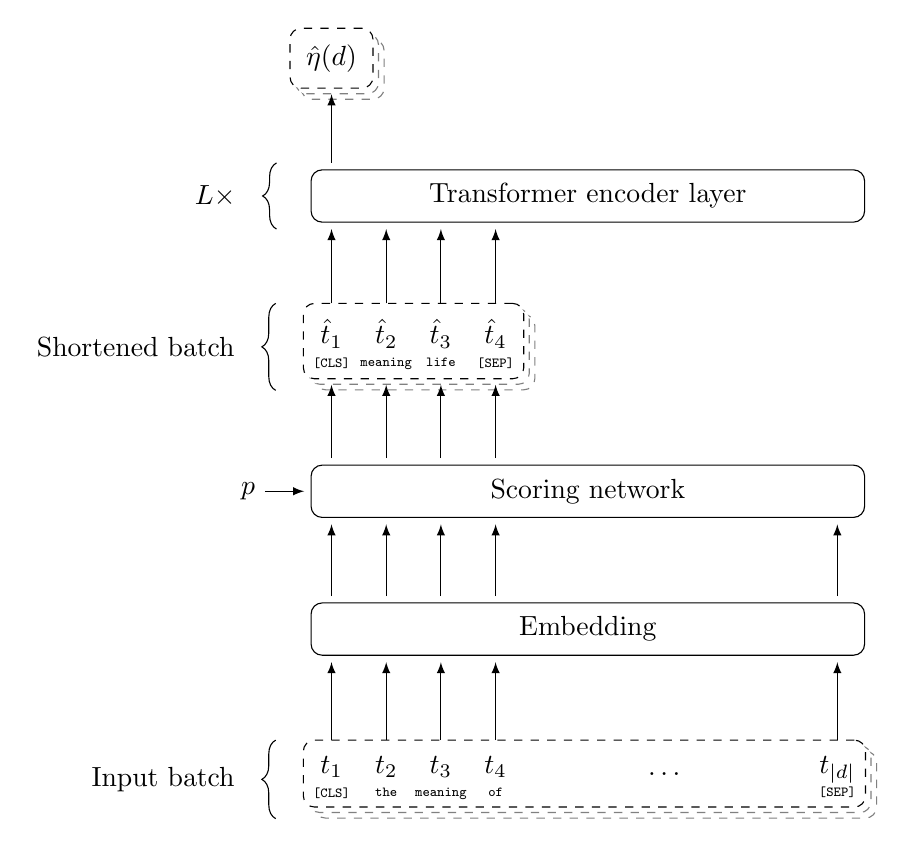
\begin{tikzpicture}
    % embedding
    \node[
        framedfignode,
        minimum width=200,
        fill=white,
    ] (E) at (0,0) {Embedding};

    % inputs
    \node[
        fignode,
        below=1.75 of E.west,
        anchor=west,
    ] (T1) {$t_1$};
    \node[
        below=-0.2 of T1,
    ] (T1b) {\tiny \texttt{[CLS]}};

    \node[
        fignode,
        right=0 of T1,
        anchor=west,
    ] (T2) {$t_2$};
    \node[
        below=-0.2 of T2,
    ] (T2b) {\tiny \texttt{the}};

    \node[
        fignode,
        right=0 of T2,
        anchor=west,
    ] (T3) {$t_3$};
    \node[
        below=-0.2 of T3,
    ] {\tiny \texttt{meaning}};

    \node[
        fignode,
        right=0 of T3,
        anchor=west,
    ] (T4) {$t_4$};
    \node[
        below=-0.2 of T4,
    ] (T4b) {\tiny \texttt{of}};

    \node[
        fignode,
        anchor=north east,
    ] (Td) at (T4.north -| E.east) {$t_{|d|}$};
    \node (Tdb) at (Td |- T4b) {\tiny \texttt{[SEP]}};

    \node[
        fignode,
    ] at ($(T4.north)!0.5!(Tdb.south)$) {\dots};

    % scoring network
    \node[
        framedfignode,
        minimum width=200,
        above=1.75 of E.west,
        anchor=west,
        fill=white,
    ] (S) {Scoring network};
    \node[
        left=0.5 of S,
    ] (P) {$p$};
    \draw[-latex] (P) -- (S);

    % intermediate representations
    \node[
        fignode,
        above=2 of S.west,
        anchor=west,
    ] (Ts1) {$\hat{t}_1$};
    \node[
        below=-0.2 of Ts1,
    ] (Ts1b) {\tiny \texttt{[CLS]}};

    \node[
        fignode,
        right=0 of Ts1,
        anchor=west,
    ] (Ts2) {$\hat{t}_2$};
    \node[
        below=-0.2 of Ts2,
    ] (Ts2b) {\tiny \texttt{meaning}};

    \node[
        fignode,
        right=0 of Ts2,
        anchor=west,
    ] (Ts3) {$\hat{t}_3$};
    \node[
        below=-0.2 of Ts3,
    ] (Ts3b) {\tiny \texttt{life}};

    \node[
        fignode,
        right=0 of Ts3,
        anchor=west,
    ] (Ts4) {$\hat{t}_4$};
    \node[
        below=-0.2 of Ts4,
    ] (Ts4b) {\tiny \texttt{[SEP]}};

    % encoder
    \node[
        framedfignode,
        minimum width=200,
        above=1.75 of Ts1.west,
        anchor=west,
        fill=white,
    ] (L) {Transformer encoder layer};

    % output
    \node[
        fignode,
        above=1.75 of L -| T1,
        anchor=center,
    ] (O) {$\hat{\eta}(d)$};

    % batch visualization
    \begin{scope}[on background layer]
        \node[
            xshift=4,
            yshift=-4,
            fit=(T1b.south west |- T1.north west)(Tdb.south east),
            inner sep=0,
            dashed,
            rounded corners,
            draw=gray,
            fill=white,
        ] (Tr) {};
        \node[
            xshift=2,
            yshift=-2,
            fit=(T1b.south west |- T1.north west)(Tdb.south east),
            inner sep=0,
            dashed,
            rounded corners,
            fill=white,
            draw=gray,
        ] {};
        \node[
            fit=(T1b.south west |- T1.north west)(Tdb.south east),
            inner sep=0,
            dashed,
            rounded corners,
            fill=white,
            draw,
        ] {};

        \node[
            xshift=4,
            yshift=-4,
            fit=(Ts1b.south west |- Ts1.north west)(Ts4b.south east),
            inner sep=0,
            dashed,
            rounded corners,
            draw=gray,
            fill=white,
        ] (Tsr) {};
        \node[
            xshift=2,
            yshift=-2,
            fit=(Ts1b.south west |- Ts1.north west)(Ts4b.south east),
            inner sep=0,
            dashed,
            rounded corners,
            fill=white,
            draw=gray,
        ] (Tsm) {};
        \node[
            fit=(Ts1b.south west |- Ts1.north west)(Ts4b.south east),
            inner sep=0,
            dashed,
            rounded corners,
            fill=white,
            draw,
        ] {};

        \node[
            xshift=4,
            yshift=-4,
            fit=(O),
            inner sep=0,
            dashed,
            rounded corners,
            draw=gray,
            fill=white,
        ] {};
        \node[
            xshift=2,
            yshift=-2,
            fit=(O),
            inner sep=0,
            dashed,
            rounded corners,
            fill=white,
            draw=gray,
            fill=white,
        ] (Om) {};
        \node[
            fit=(O),
            inner sep=0,
            dashed,
            rounded corners,
            fill=white,
            draw,
        ] {};
    \end{scope}

    % inputs -> embedding
    \draw[-latex] (T1) -- (T1 |- E.south);
    \draw[-latex] (T2) -- (T2 |- E.south);
    \draw[-latex] (T3) -- (T3 |- E.south);
    \draw[-latex] (T4) -- (T4 |- E.south);
    \draw[-latex] (Td) -- (Td |- E.south);

    % embedding -> scoring network
    \draw[-latex] (E.north -| T1) -- (S.south -| T1);
    \draw[-latex] (E.north -| T2) -- (S.south -| T2);
    \draw[-latex] (E.north -| T3) -- (S.south -| T3);
    \draw[-latex] (E.north -| T4) -- (S.south -| T4);
    \draw[-latex] (E.north -| Td) -- (S.south -| Td);

    % scoring network -> intermediate representations
    \draw[-latex] (S.north -| Ts1) -- (Ts1b |- Tsm.south);
    \draw[-latex] (S.north -| Ts2) -- (Ts2b |- Tsm.south);
    \draw[-latex] (S.north -| Ts3) -- (Ts3b |- Tsm.south);
    \draw[-latex] (S.north -| Ts4) -- (Ts4b |- Tsm.south);

    % intermediate representations -> encoder
    \draw[-latex] (Ts1) -- (L.south -| Ts1);
    \draw[-latex] (Ts2) -- (L.south -| Ts2);
    \draw[-latex] (Ts3) -- (L.south -| Ts3);
    \draw[-latex] (Ts4) -- (L.south -| Ts4);

    % encoder -> output
    \draw[-latex] (L.north -| T1) -- (Om.south -| T1);

    % annotations
    \draw [
        decorate,
        decoration={
                brace,
                raise=10,
                amplitude=5,
            },
    ] (T1b.south west |- Tr.south) -- (T1.north west -| T1b.south west) node[left=0.75,midway] {Input batch};

    \draw [
        decorate,
        decoration={
                brace,
                raise=10,
                amplitude=5,
            },
    ] (Ts1b.south west |- Tsr.south) -- (Ts1.north west -| Ts1b.south west) node[left=0.75,midway] {Shortened batch};

    \draw [
        decorate,
        decoration={
                brace,
                raise=10,
                amplitude=5,
            },
    ] (L.south west) -- (L.north west) node[left=0.75,midway] {$L \times$};
\end{tikzpicture}
\end{document}
